\chapter{Diseño de la plataforma web interactiva}
\label{cap:web}

Como parte del trabajo se ha desarrollado una aplicación web interactiva. Su papel es ayudar a explorar, explicar y probar el detector desde una interfaz visual, sin sustituir a la evaluación experimental del Capítulo~\ref{cap:experimentos}. En este capítulo se describe su objetivo, su arquitectura, sus partes principales y sus limitaciones.

\section{Objetivo de la aplicación}
\label{sec:web_objetivo}

El detector y sus resultados viven, sobre todo, en scripts, ficheros CSV y tablas. Eso es suficiente para evaluarlo, pero no para entenderlo de un vistazo. La aplicación web cubre ese hueco: pone delante de una persona, de forma visual, qué familias de ataque se estudian, cómo se comporta cada una, qué señales mira el detector y por qué toma cada decisión.

En concreto, la web permite explorar las familias de ataque y su patrón de comportamiento, consultar las explicaciones del detector con las señales que usa y una regla simplificada, generar ventanas de tráfico sintéticas para ver la forma de cada ataque y probar el clasificador subiendo un fichero pequeño y viendo su salida traza a traza.

La web es una herramienta de visualización, explicación y prueba, no el sistema de evaluación. Las métricas del Capítulo~\ref{cap:experimentos} se calculan con los scripts del proyecto, no desde la interfaz. La web ayuda a interpretar esos resultados y a probar el detector en casos pequeños, pero no los reemplaza.

\section{Arquitectura general}
\label{sec:web_arquitectura}

La aplicación se divide en dos partes. Un \textbf{frontend} web que es lo que ve el usuario, y un \textbf{backend} que sirve los datos y ejecuta las operaciones que no pueden hacerse en el navegador. El frontend pide información al backend mediante llamadas HTTP a una API, y el backend responde con datos en formato JSON.

Los datos que muestra la web (la información de cada ataque, sus señales y sus métricas) están en ficheros estáticos pequeños que el backend lee y expone a través de la API. Para las funciones que necesitan cálculo (generar una ventana sintética o clasificar un fichero), el frontend llama a un endpoint y el backend hace el trabajo. La integración con NotebookLM es opcional y solo se activa en el modo IA ON, como se explica más adelante.

\begin{figure}[ht]
\centering
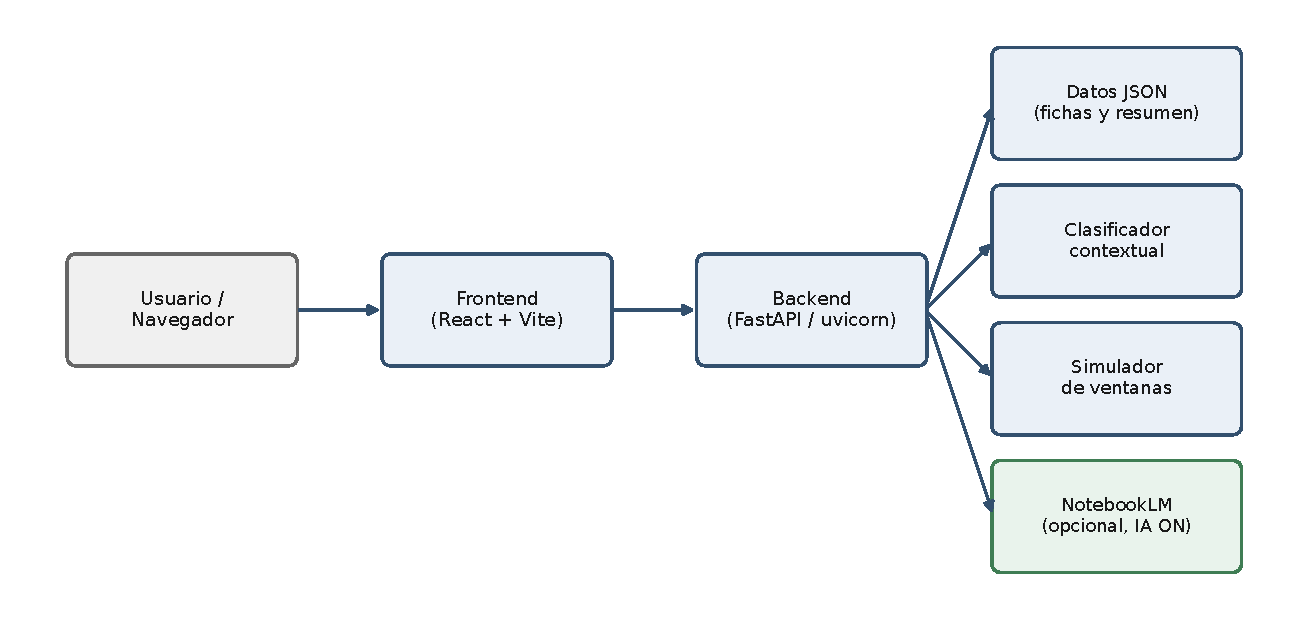
\includegraphics[width=\textwidth]{imagenes/fig_arquitectura_web.pdf}
\caption{Arquitectura general de la aplicación web: frontend, backend, datos del proyecto, simulador, clasificador y módulo opcional de NotebookLM.}
\label{fig:arquitectura_web}
\end{figure}

\section{Frontend}
\label{sec:web_frontend}

El frontend está construido con \textbf{React} (versión 18) y empaquetado con \textbf{Vite}. No usa ninguna librería de enrutado externa: la navegación entre la portada y la página de cada ataque se hace por \emph{hash} en la URL (rutas del tipo \texttt{\#/attacks/<id>}). El estado del modo IA se guarda en el almacenamiento local del navegador, de modo que se mantiene entre páginas.

La interfaz tiene dos pantallas principales. La \textbf{portada} muestra las familias de ataque como burbujas flotantes sobre las que se puede pulsar, y debajo unas secciones compactas con el funcionamiento del clasificador v5, un resumen de resultados, las comparaciones y la evolución de versiones. La \textbf{página de ataque} muestra una sola familia con su descripción, un diagrama del patrón, las señales que usa el detector, una regla simplificada, sus métricas y sus limitaciones.

Los componentes principales son la portada (\texttt{Home}), la zona flotante de ataques (\texttt{FloatingAttacks}), la página de detalle (\texttt{AttackDetail}) con su diagrama (\texttt{AttackDiagram}), el simulador de ventanas (\texttt{AttackSimulator}), el chat contextual (\texttt{FloatingAttackChat}), el ejecutor del clasificador (\texttt{ClassifierRunner}) y el interruptor del modo IA (\texttt{AiToggle}). Los textos didácticos de cada ataque están en un fichero de metadatos del propio frontend, mientras que los datos duros (métricas, patrón, limitaciones) vienen del backend.

\section{Backend}
\label{sec:web_backend}

El backend está construido con \textbf{FastAPI} y se ejecuta con el servidor \texttt{uvicorn}. Su versión base es deliberadamente sencilla: lee ficheros JSON pequeños de la carpeta de datos y los expone como API, sin cargar los CSV grandes del dataset. La API ofrece, entre otros, los siguientes endpoints:

\begin{itemize}
  \item \texttt{GET /api/health} y \texttt{GET /api/summary}, para el estado del servicio y el resumen del proyecto.
  \item \texttt{GET /api/attacks} y \texttt{GET /api/attacks/\{id\}}, para el listado de familias y la ficha de cada una.
  \item \texttt{GET /api/ai/status}, que indica si el modo IA ON está disponible sin exponer credenciales.
  \item \texttt{POST /api/simulator/generate}, que genera una ventana sintética de un ataque.
  \item \texttt{POST /api/notebooklm/chat}, que envía una pregunta al cuaderno de NotebookLM del ataque (solo en modo IA ON).
  \item \texttt{GET /api/classifier/expected-columns} y \texttt{POST /api/classifier/run}, para conocer las columnas esperadas y clasificar una ventana subida por el usuario.
\end{itemize}

Además, el backend sirve el frontend ya compilado, de forma que toda la aplicación queda accesible desde una sola dirección. La ejecución del clasificador desde la web reutiliza la lógica de la versión v3 más el tercer pase de la v5, pero está pensada para ficheros pequeños. La validación científica completa sigue estando en los scripts de análisis, no en la web.

\section{Datos utilizados por la web}
\label{sec:web_datos}

La web no usa los CSV grandes del dataset. Toda la información que muestra está en dos ficheros JSON pequeños. El primero contiene la ficha de cada familia de ataque: nombre, familia conductual, descripción, patrón técnico, señales que usa el detector, métricas y limitaciones. El segundo contiene un resumen del proyecto: enfoque, metodología, comparación con ML clásico y limitaciones generales.

Estos datos son los que alimentan tanto la portada como las páginas de ataque. Las familias incluidas son las seis activas del trabajo (\texttt{scan11}, \texttt{scan44}, \texttt{anomaly-udpscan}, \texttt{dos}, \texttt{nerisbotnet} y \texttt{anomaly-sshscan}). La clase de campaña SMTP (\texttt{anomaly-spam}) se retiró de los resultados activos, como se explicó en capítulos anteriores, y no aparece en la web. Solo se conserva como material histórico fuera de la aplicación.

\section{Visualización de familias de ataque}
\label{sec:web_visualizacion}

La Figura~\ref{fig:web_principal} muestra la pantalla principal de la aplicación, desde la que se accede a las familias de ataque y a las funciones generales del sistema.

\begin{figure}[!htbp]
\centering
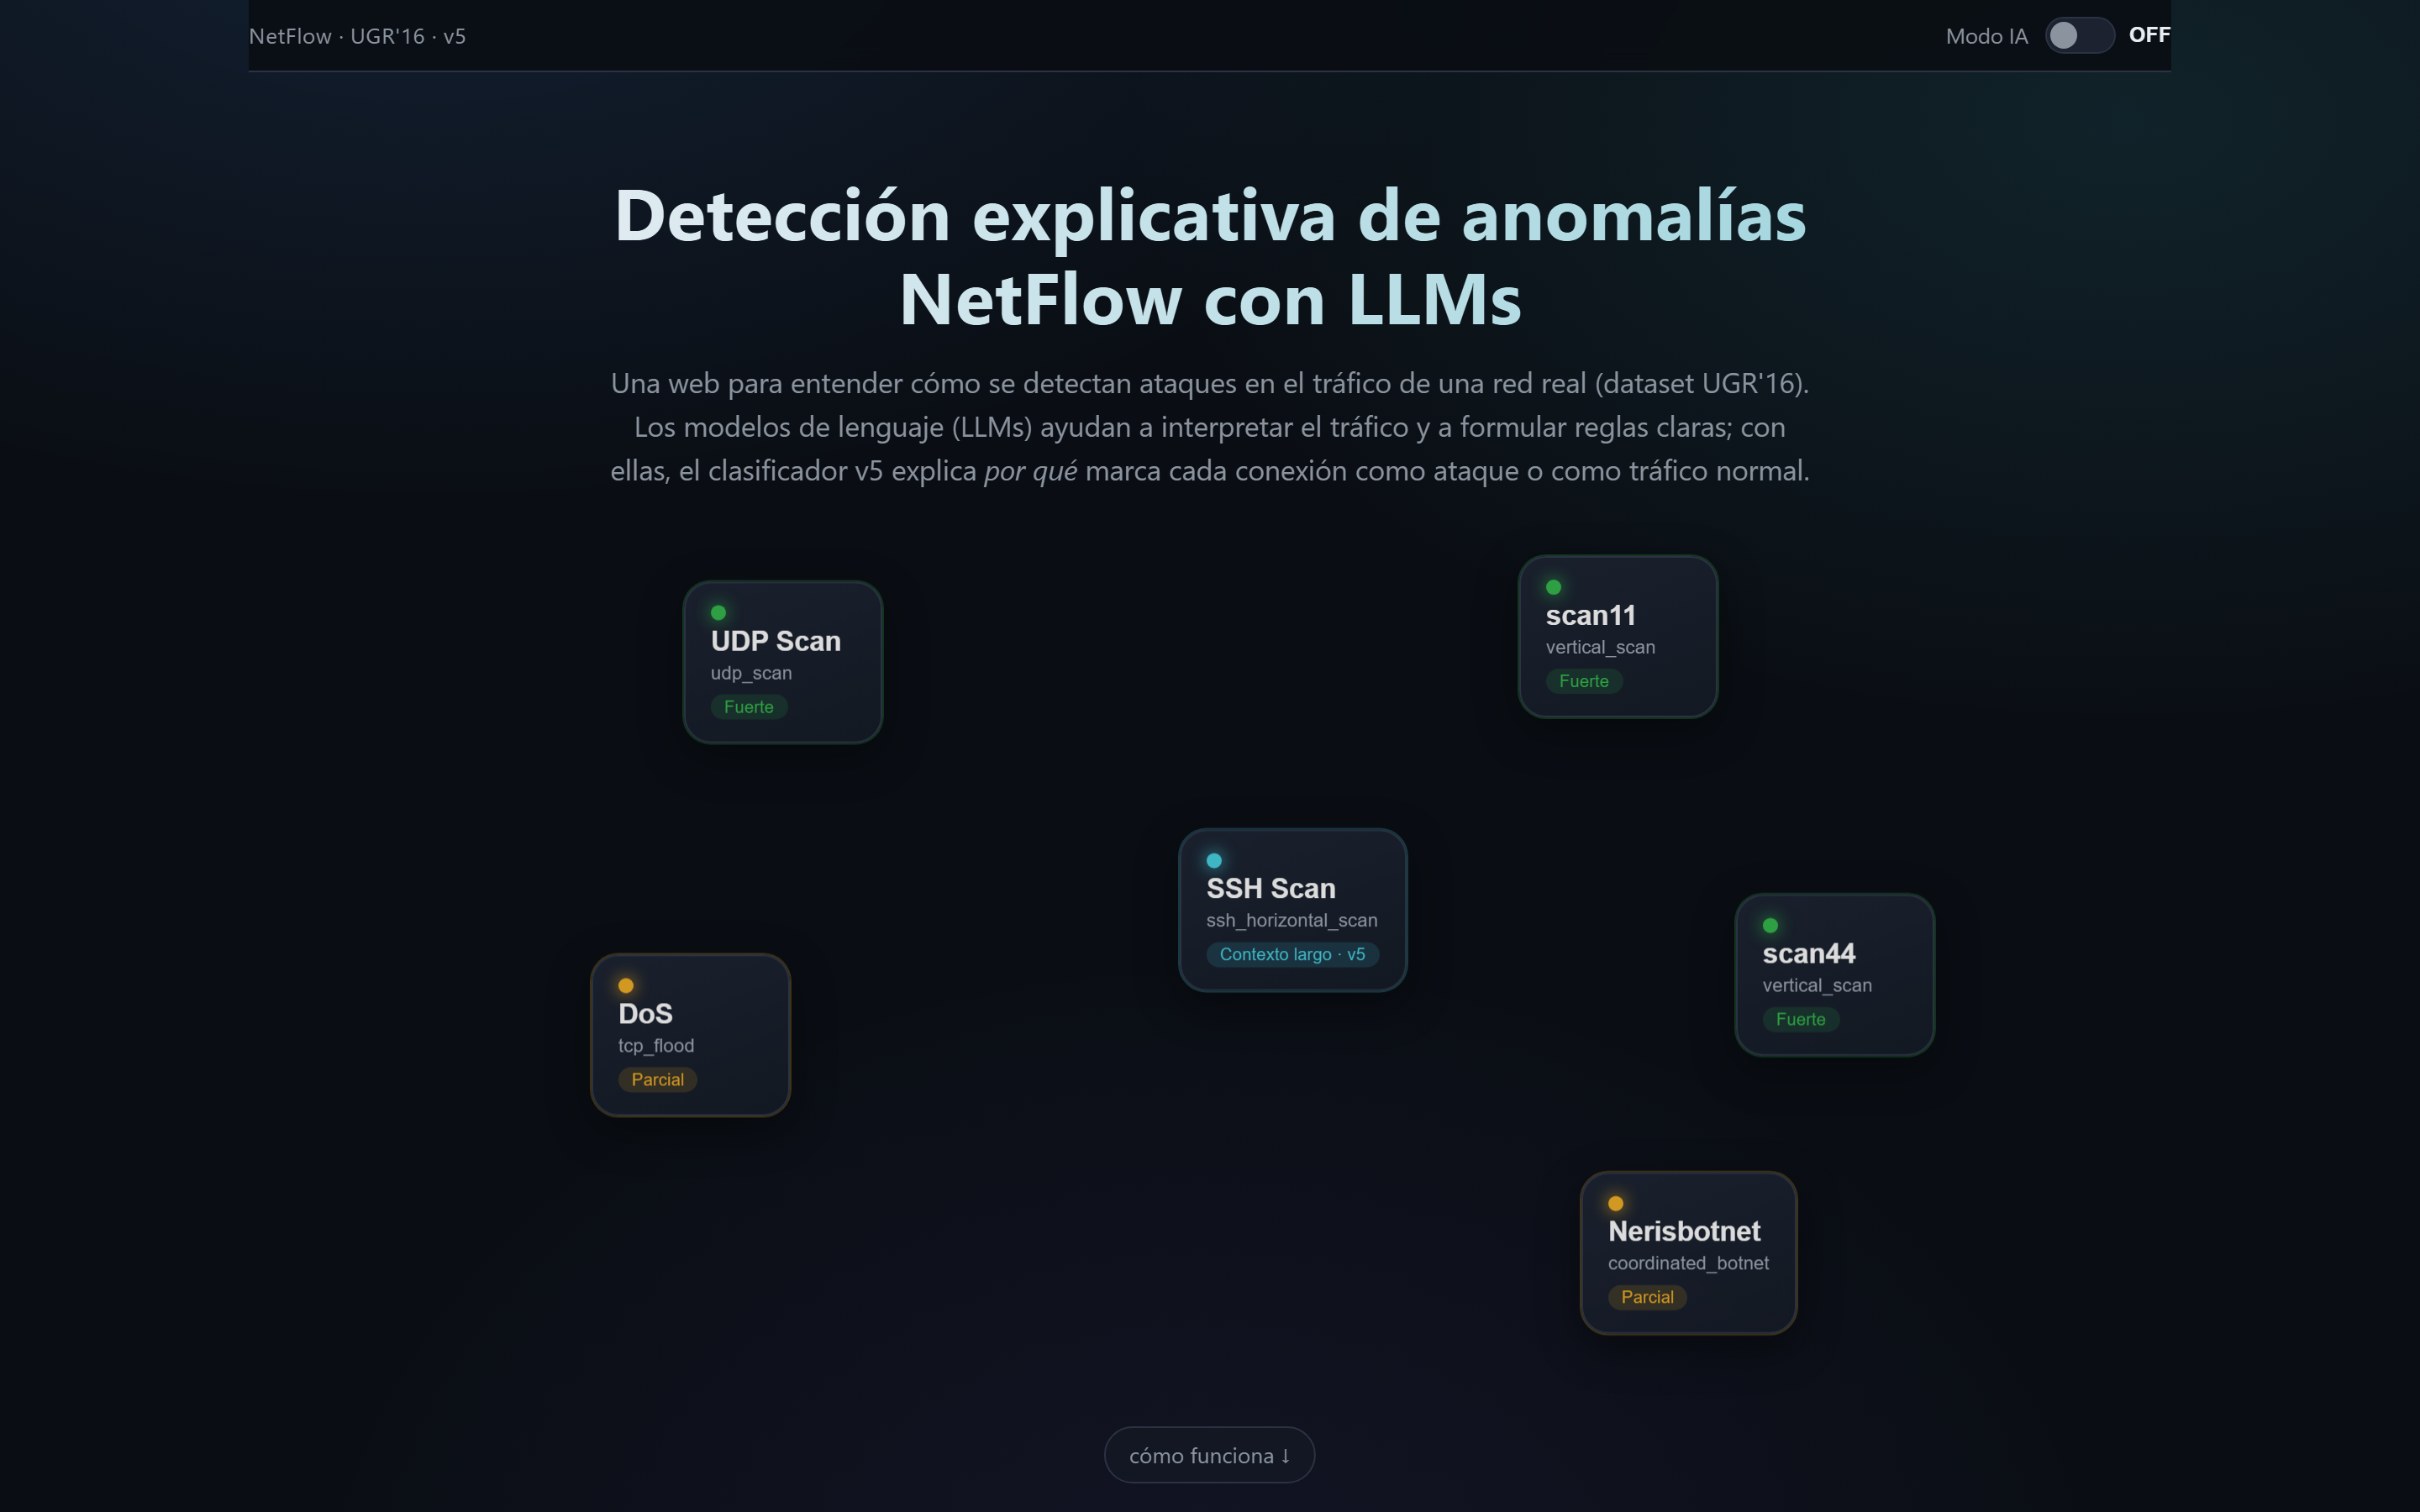
\includegraphics[width=0.9\textwidth]{imagenes/web_pantalla_principal.png}
\caption{Pantalla principal de la aplicación web, desde la que se accede a las familias de ataque y a las principales funciones del sistema.}
\label{fig:web_principal}
\end{figure}

Cuando el usuario pulsa sobre una familia, la web abre su página de detalle (Figura~\ref{fig:web_detalle}). Allí se muestra, para esa familia, la descripción del ataque, un diagrama del patrón, una explicación en lenguaje sencillo, las características que mira el detector (cada señal con qué mide y por qué importa), los pasos de detección, una regla simplificada en forma de pseudocódigo, lo que el detector \emph{no} usa, sus métricas con su significado, el contexto de validación y sus limitaciones.

\begin{figure}[!htbp]
\centering
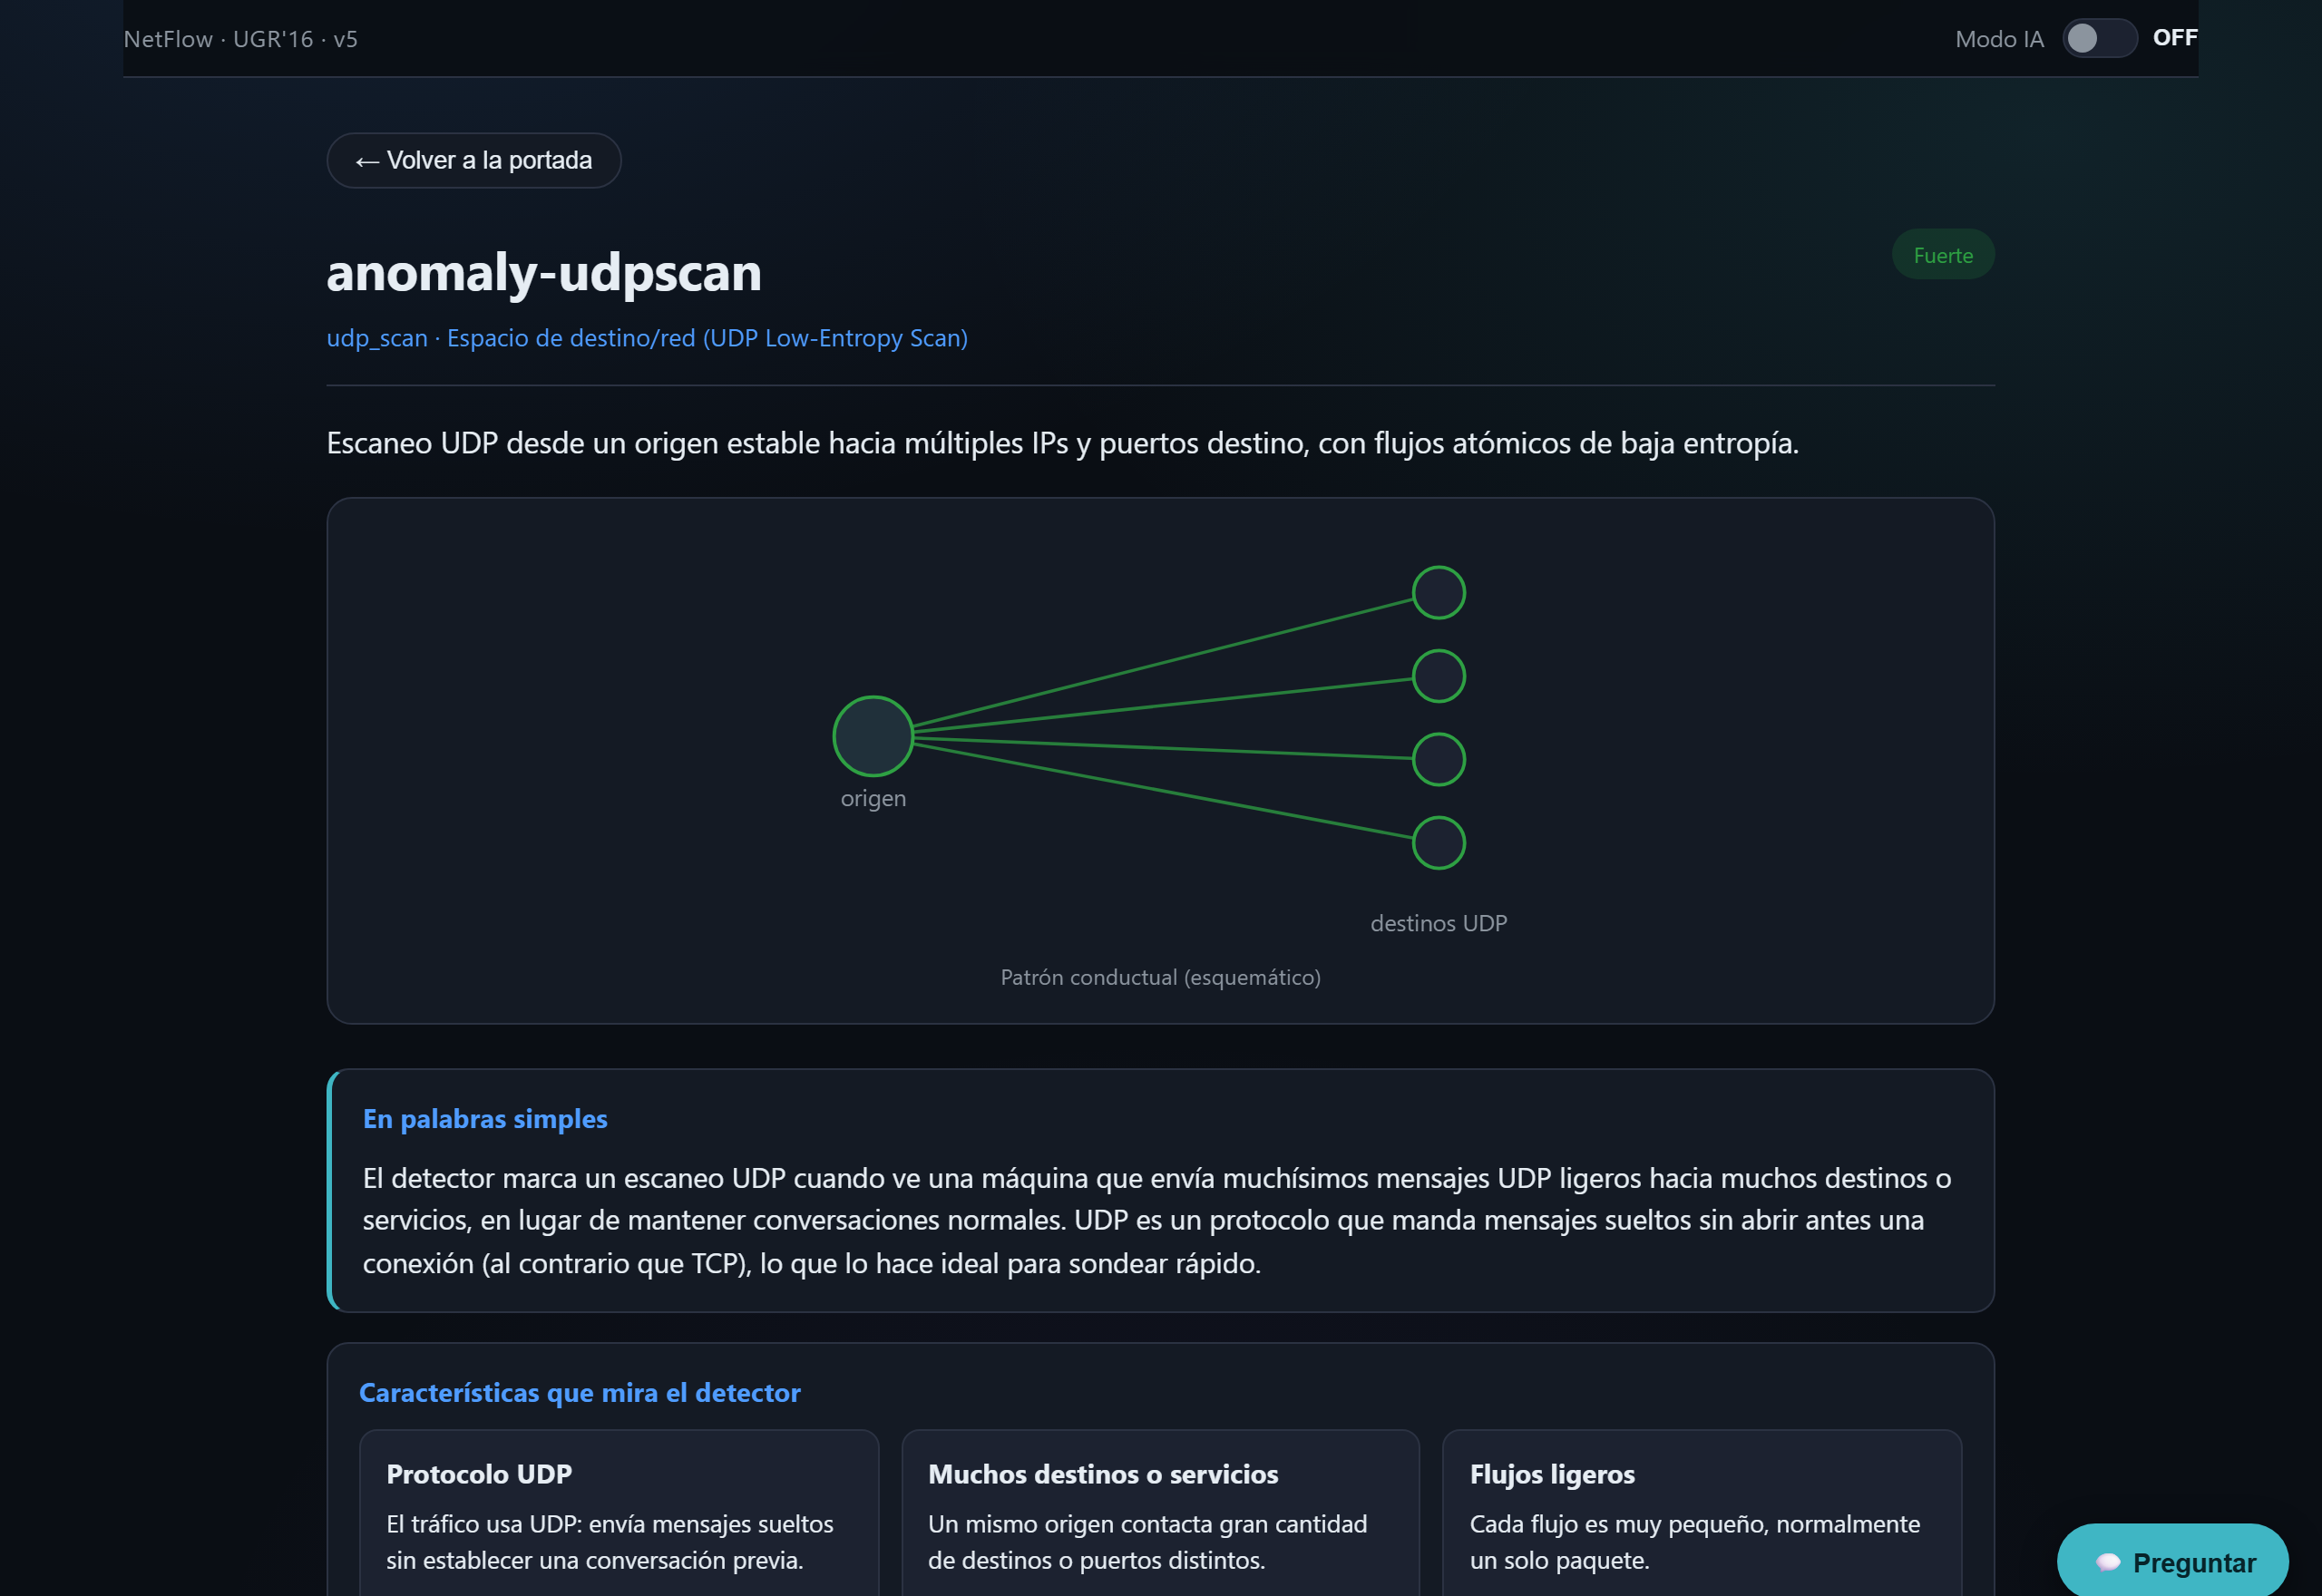
\includegraphics[width=0.9\textwidth]{imagenes/web_detalle_familia.png}
\caption{Pantalla de detalle de una familia de ataque en la aplicación web.}
\label{fig:web_detalle}
\end{figure}

La idea es que cualquier persona con formación en informática, aunque no sea especialista en seguridad, pueda entender por qué el detector marca un ataque. Por eso las señales se explican con palabras y no solo con fórmulas, y la regla se presenta de forma ilustrativa, no como el código real. Las métricas que se muestran son las mismas que se documentan en el Capítulo~\ref{cap:experimentos}. La Figura~\ref{fig:web_senales} recoge cómo presenta la web esas señales conductuales.

\begin{figure}[!htbp]
\centering
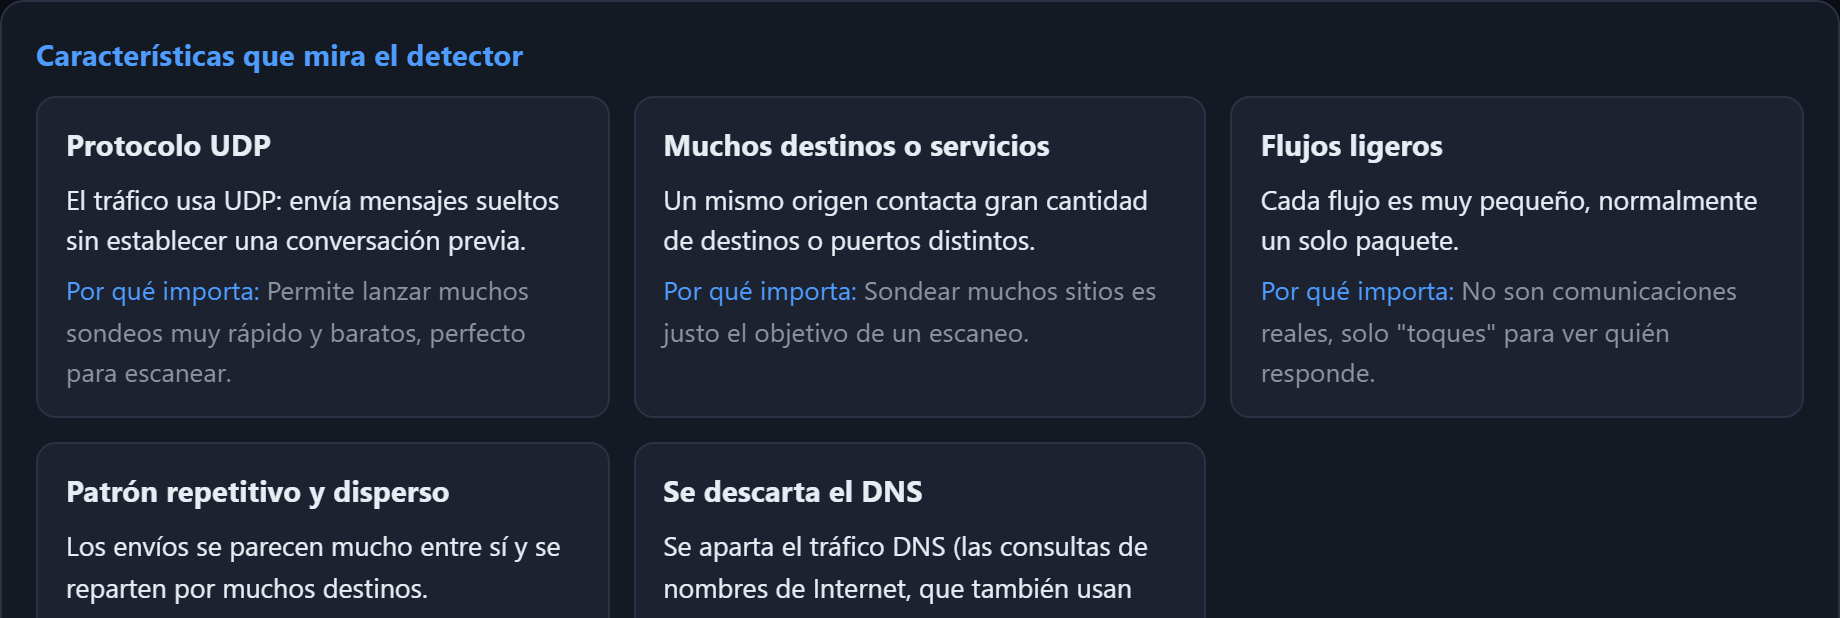
\includegraphics[width=0.9\textwidth]{imagenes/web_senales_detector.png}
\caption{Señales conductuales mostradas por la web para explicar la decisión del detector.}
\label{fig:web_senales}
\end{figure}

\section{Simulación de ventanas sintéticas}
\label{sec:web_simulador}

Cada página de ataque incluye un simulador. Al pulsar un botón, la web genera una ventana de tráfico sintética con la forma de ese ataque: unas pocas trazas normales antes, las trazas del ataque en medio y unas pocas trazas normales después. El usuario puede elegir cuántas trazas de ataque generar y descargar el resultado en formato CSV.

Estos datos son sintéticos e ilustrativos. No son trazas reales del dataset, sino ejemplos creados para ver el patrón de cada ataque. Sirven para entender la forma del comportamiento (cuántos destinos, qué puertos, qué concentración o dispersión), no para evaluar el detector. Cada generación produce una variante distinta del mismo patrón, de modo que se aprecia que el ataque no depende de una IP concreta, sino de su estructura.

En el modo IA OFF, el simulador usa plantillas locales sencillas de la propia web. No se emplea ningún mecanismo de generación reproducible por semilla. La validación real del detector se hizo siempre con UGR'16, no con estas ventanas.

\begin{figure}[ht]
\centering
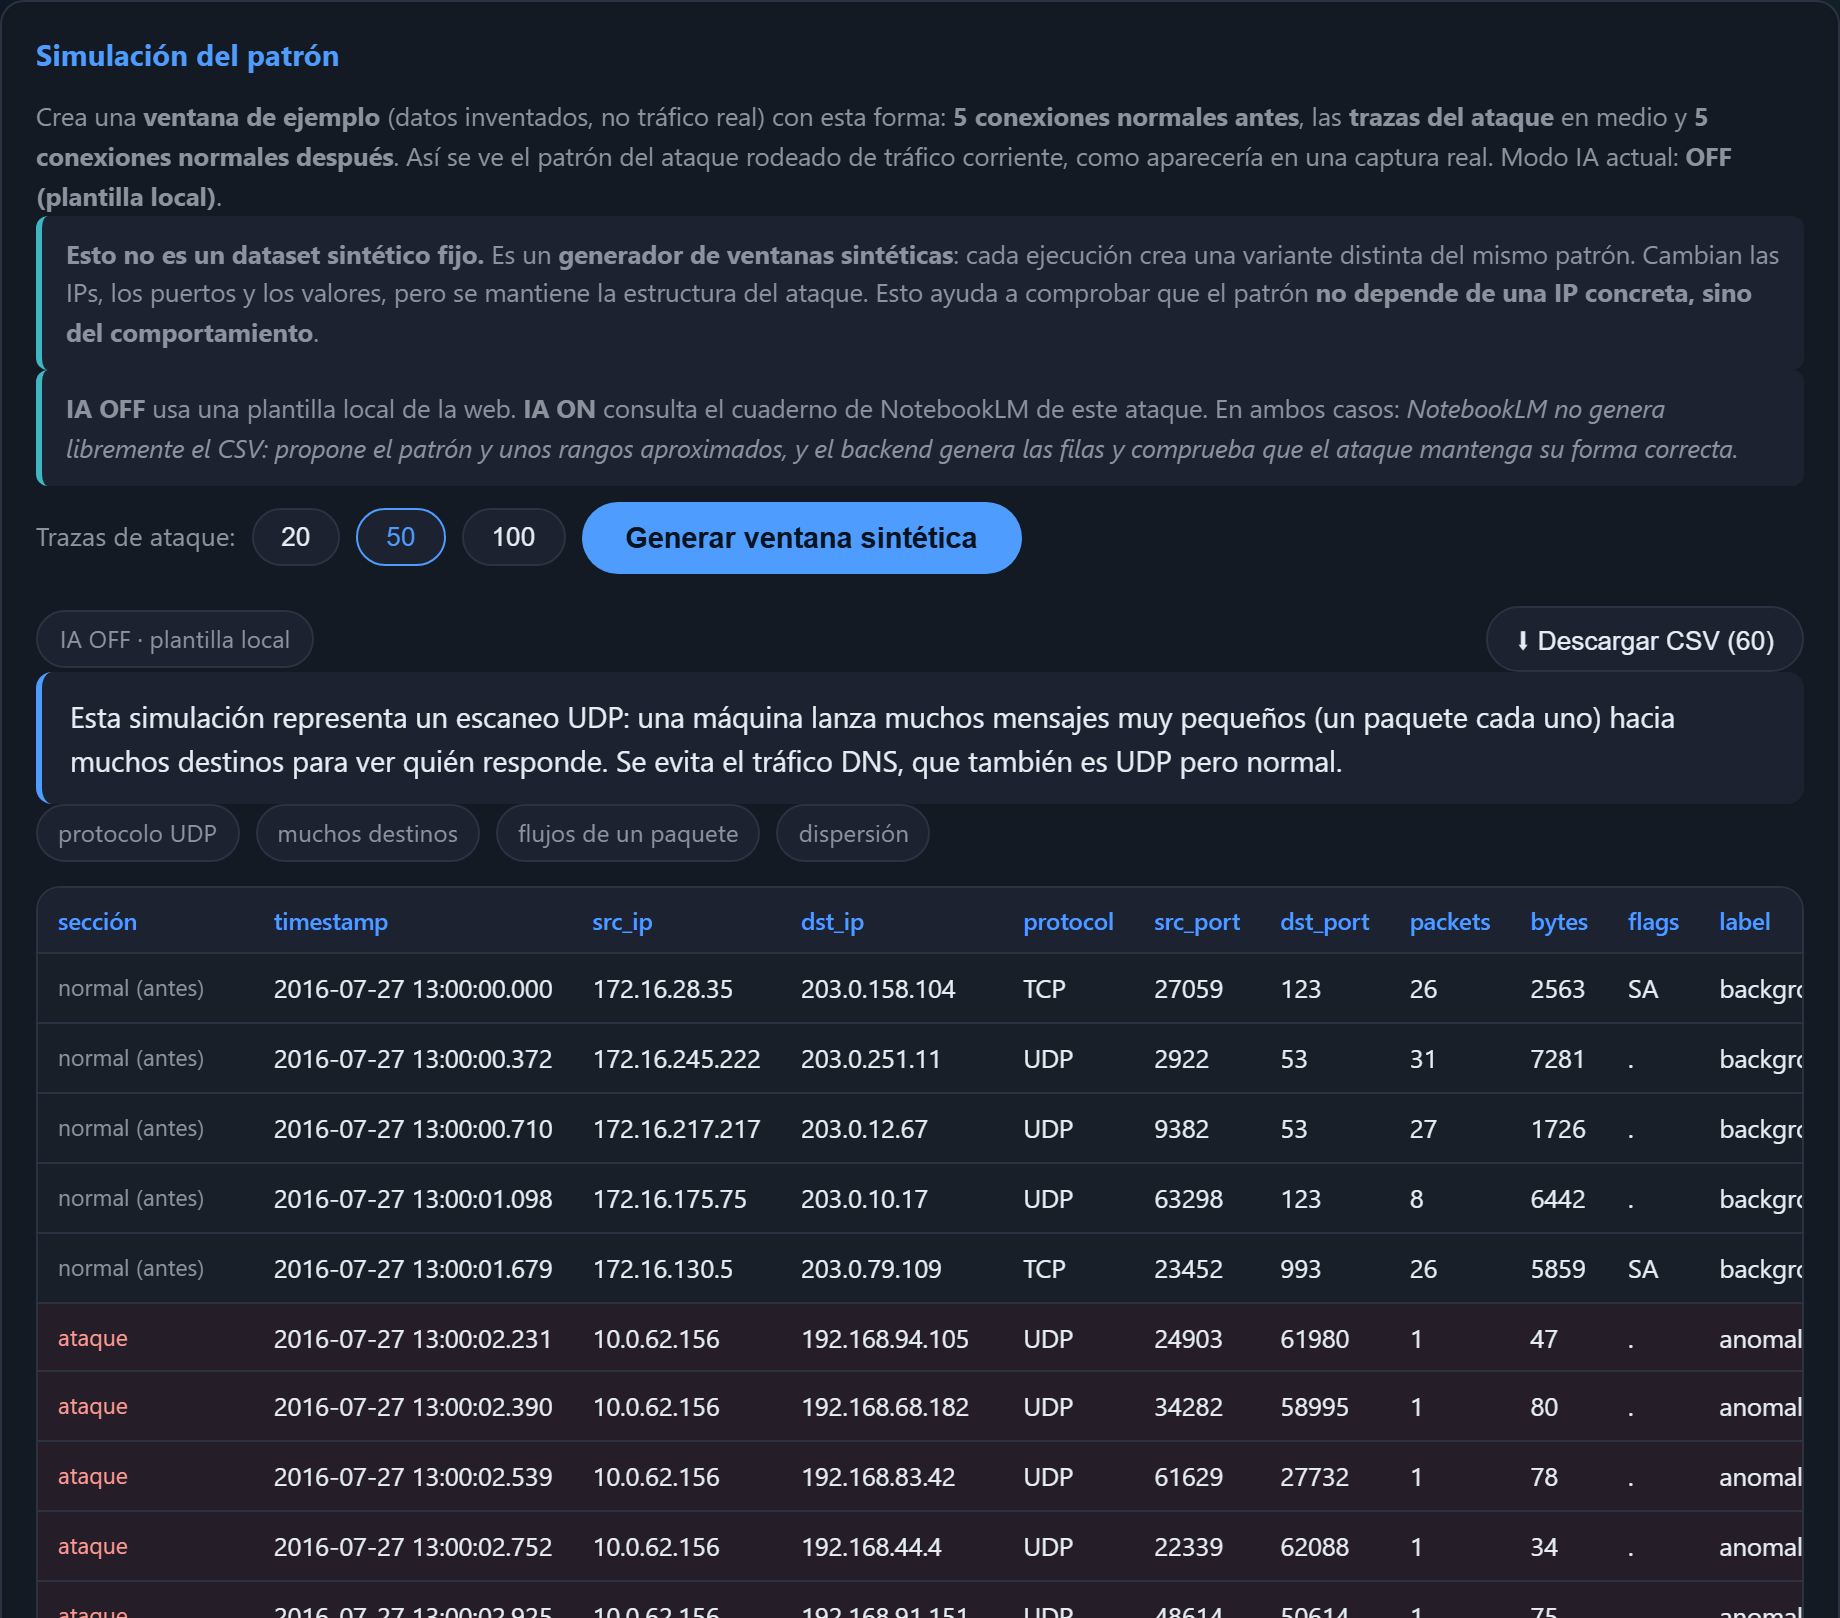
\includegraphics[width=0.9\textwidth]{imagenes/web_simulador.png}
\caption{Simulador de ventanas sintéticas utilizado para ilustrar patrones de ataque.}
\label{fig:web_simulador}
\end{figure}

\section{Modo IA y uso de NotebookLM}
\label{sec:web_ia}

La web tiene un interruptor global de modo IA, con dos estados. En el modo \textbf{IA OFF}, que es el de por defecto, todo funciona en local: las explicaciones y las simulaciones usan plantillas y textos de la propia web, sin conexión externa. En el modo \textbf{IA ON}, algunas funciones se apoyan en NotebookLM \cite{notebooklm}.

El uso de NotebookLM es un \textbf{modo experimental} y un \textbf{apoyo auxiliar}. Sirve para dos cosas: un chat por ataque, que ayuda a generar o consultar explicaciones, y la propuesta de patrones para el simulador. En ningún caso NotebookLM detecta ataques ni decide nada. La detección la hace siempre el clasificador de reglas, y NotebookLM \textbf{no interviene en el cálculo de las métricas del Capítulo~\ref{cap:experimentos}}.

Esta integración depende de configuración local. Necesita que se hayan configurado los cuadernos de cada ataque y las credenciales correspondientes en variables de entorno que no se versionan, además de la biblioteca cliente instalada y una sesión válida. No es una integración oficial de NotebookLM, sino un uso a través de una biblioteca cliente. Si el modo IA ON no está disponible para un ataque, o si tarda o falla, la web lo avisa y vuelve automáticamente al modo IA OFF, de modo que la aplicación sigue siendo usable en todo momento.

\section{Ejecución del clasificador desde la web}
\label{sec:web_clasificador}

La web permite probar el clasificador sin tocar los scripts. El usuario sube una ventana en formato CSV (con un límite de tamaño pequeño, de unos pocos megabytes), la web comprueba que tenga las columnas esperadas y la envía al backend, que ejecuta el clasificador sobre cada traza. La respuesta incluye, por traza, la decisión (ataque o normal), la familia, el subtipo, un nivel de confianza y la señal que ha justificado la decisión, junto con un resumen del conjunto (Figura~\ref{fig:web_clasificador}).

\begin{figure}[!htbp]
\centering
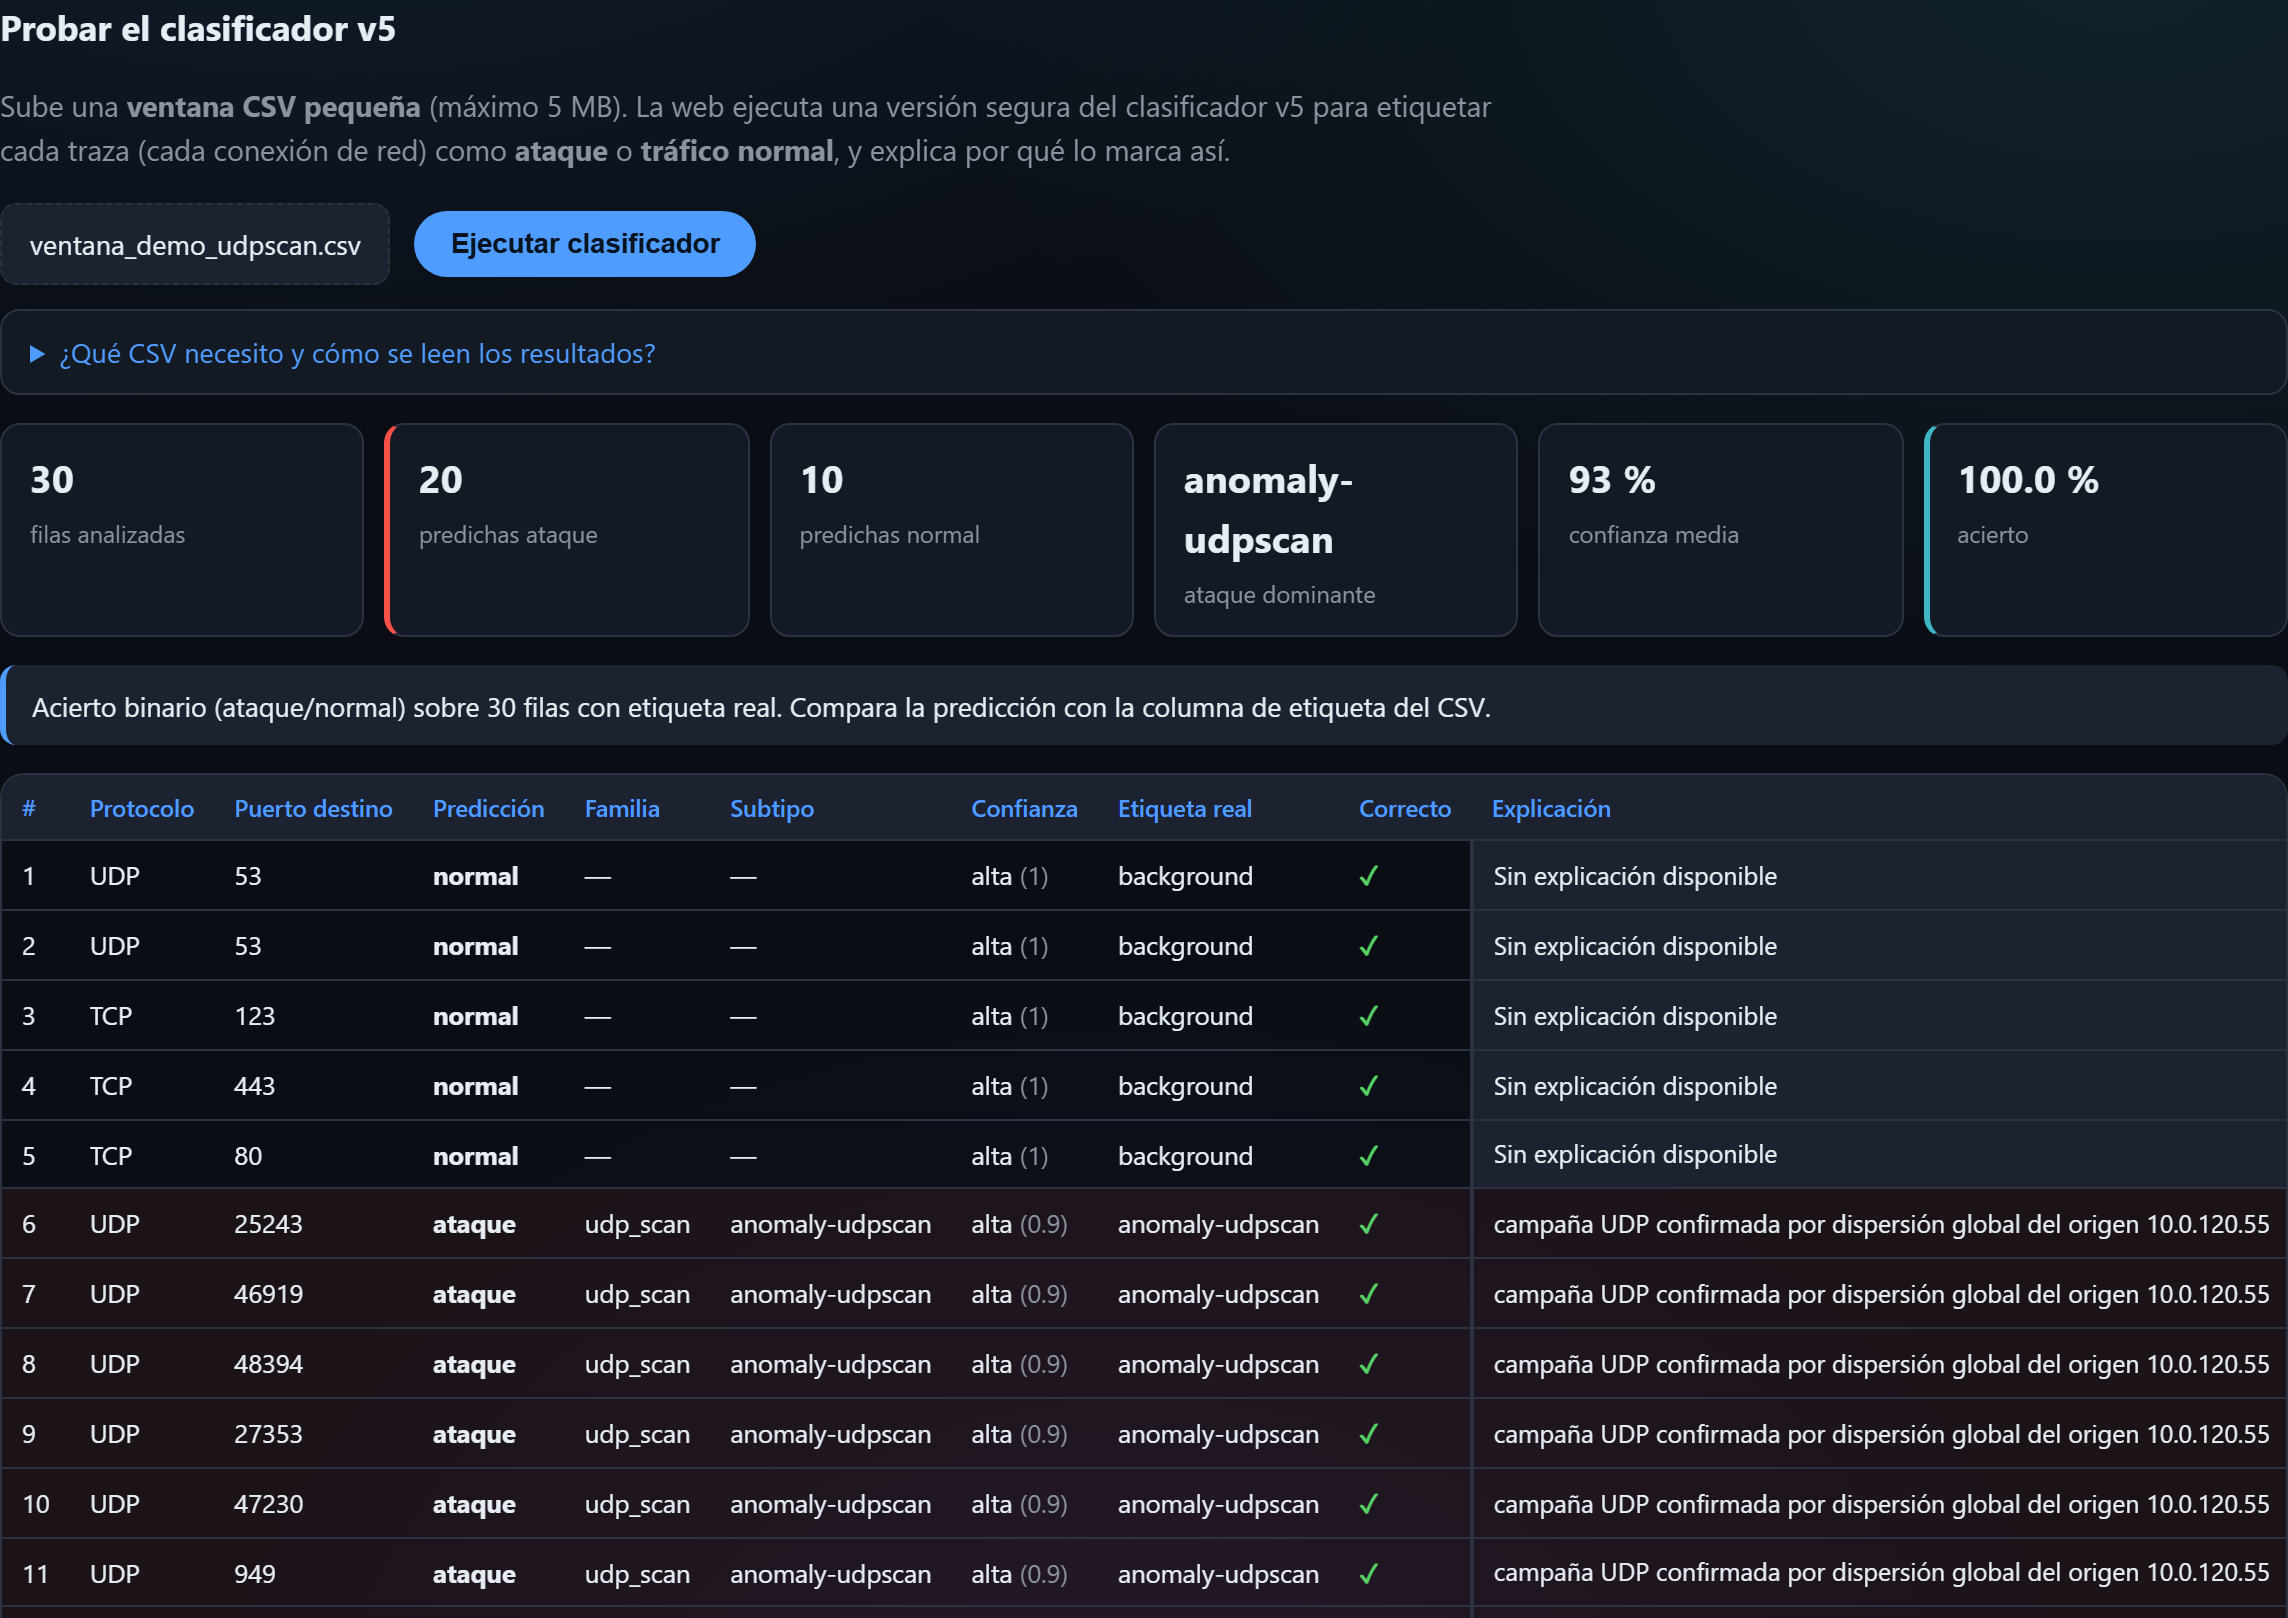
\includegraphics[width=0.9\textwidth]{imagenes/web_clasificador.png}
\caption{Ejecución del clasificador contextual desde la aplicación web sobre un CSV pequeño de ejemplo.}
\label{fig:web_clasificador}
\end{figure}

La interfaz distingue con cuidado dos cosas que es fácil confundir. La \textbf{confianza} es la fuerza de la evidencia de la regla, no una probabilidad de un modelo. El \textbf{acierto} solo puede calcularse si el CSV incluye la etiqueta real. Si no la trae, la web muestra solo la confianza y lo indica, sin inventar un porcentaje de acierto.

Esta función está pensada para pruebas pequeñas o de demostración. No procesa el dataset completo ni grandes volúmenes desde la interfaz, que es justo el trabajo que hacen los scripts de análisis del Capítulo~\ref{cap:experimentos}.

\section{Despliegue y ejecución}
\label{sec:web_despliegue}

Durante el desarrollo, el frontend y el backend se ejecutan por separado: el frontend con el servidor de desarrollo de Vite y el backend con \texttt{uvicorn}. Para usar la aplicación como un todo, el frontend se compila y el backend sirve el resultado, de forma que toda la web queda detrás de una sola dirección.

Para poder abrir la web desde otro ordenador sin desplegarla en un servidor permanente, se usa un túnel de Cloudflare (\texttt{cloudflared}), que expone temporalmente la aplicación local en una URL pública del tipo \texttt{https://...trycloudflare.com}. Es una solución pensada para pruebas y demostración, no para un despliegue en producción.

La configuración sensible (los identificadores de los cuadernos de NotebookLM y las credenciales) se guarda en un fichero de variables de entorno que no se versiona, de modo que no aparece ninguna clave ni token en el código del proyecto. Los pasos concretos para lanzar la web están recogidos en la guía de lanzamiento del proyecto.

\section{Limitaciones de la aplicación}
\label{sec:web_limitaciones}

La aplicación tiene límites:

\begin{itemize}
  \item No procesa datasets grandes desde la interfaz. El clasificador web está pensado para ficheros pequeños, de prueba o demostración.
  \item No sustituye al pipeline experimental. Las métricas y la evaluación se obtienen con los scripts, no con la web.
  \item El modo IA ON depende de configuración local. NotebookLM puede no estar disponible, tardar unos segundos o fallar, y en ese caso la web cae al modo IA OFF.
  \item Las simulaciones son ilustrativas. Sirven para entender los patrones, no para medir el rendimiento del detector.
  \item El modo IA ON necesita un cliente de NotebookLM instalado aparte (dependencia opcional) y configuración local. El resto de la web, incluido el clasificador y el simulador, funciona solo con las dependencias base.
\end{itemize}

Como mejoras futuras quedan, entre otras, incluir capturas y un manual de uso más completo, ampliar los usos del modo IA ON y preparar un despliegue más estable si se quisiera mantener la web accesible de forma permanente.

\section{Conclusiones del capítulo}
\label{sec:web_conclusion}

La aplicación web reúne en una sola interfaz lo descrito en este capítulo y permite entender el detector sin leer el código.

Su valor es de apoyo: ayuda a interpretar los resultados del Capítulo~\ref{cap:experimentos} y a explicar el funcionamiento del sistema, pero no es el sistema de evaluación ni un producto cerrado. Las limitaciones señaladas y las posibles mejoras se retoman en el Capítulo~\ref{cap:conclusiones}.
